\section{Problemas de otimização}

\subsection{Conceitos básicos}

A otimização, também chamada de programação, é uma área da matemática dedicada ao estudo da obtenção de ``valores ótimos'', termo que abrange grande variedade de significados. Um caso relativamente simples de problema de otimização é a determinação de máximos e mínimos em funções contínuas. Por exemplo, suponha que a função $f(x) = x^3 - 5x^2 + 3x + 100$ represente o gasto de energia com algum processo industrial, sendo $x$ um parâmetro controlável do processo. Nesta situação, a forma ótima de conduzir o processo é aquela cujo $x$ minimiza o gasto de energia $f(x)$. Em outras palavras, queremos $x^\ast$ tal que $f(x^\ast) = \min f(x)$.

Para determinar $x^\ast$, seguimos o procedimento detalhado por \textcite{STEWART2016}. Começamos calculando $f'(x)$ e $f''(x)$. Feito isso, determinamos as raízes de $f'(x)$, que, neste caso, são $x_1 = \frac{1}{3}$ e $x_2 = 3$. Por fim, calculamos $f''(x_1) = -8$ e $f''(x_2) = 8$. De $f''(x_1) < 0$ e $f''(x_2) > 0$ concluímos que $x_1$ é ponto de máximo e $x_2$ é ponto de mínimo de $f(x)$. Portanto, $x^\ast = 3$.

\begin{figure}[h]
    \centering
    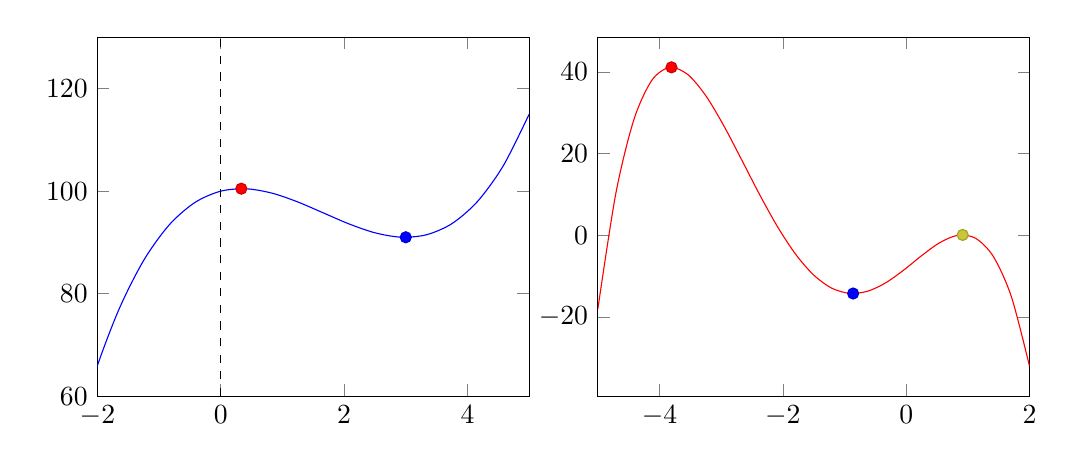
\begin{tikzpicture}
        \matrix{
            \begin{axis}[scale=0.8, xmin=-2, xmax=5, ymin=60, ymax=130]
                \addplot[color=blue,smooth]{x^3 - 5*x^2 + 3*x + 100};
                \addplot[scatter, only marks]table{
                    x y
                    0.3333 100.4815
                    3 91
                };
                \draw[dashed] (axis cs:0, 60) -- (axis cs:0, 130);
            \end{axis}
            &
            \begin{axis}[scale=0.8, xmin=-5, xmax=2]
                \addplot[color=red,smooth,domain=-5:2]{-x^4-5*x^3+2*x^2+12*x-8};
                \addplot[scatter, only marks]table{
                    x y
                    -3.80562 41.12727 
                    -0.86048 -14.20753
                    0.91611 0.12322 
                };
            \end{axis}\\
        };
    \end{tikzpicture}
    \caption{Gráficos de $f(x)$ e $g(x)$.}
    \label{fig:exemplo otimização contínua}
\end{figure}

Um leitor astuto pode perceber que $\lim_{x\to-\infty} f(x) = -\infty$; ou seja, $x$ pode ser infinitamente melhorado e, consequentemente, $x^\ast$ não existe. No entanto, isso muito provavelmente não faz sentido físico para o processo. Convém, portanto, impor uma \emph{restrição} como $x \geq 0$ ao problema. No gráfico de $f(x)$, esta restrição é a reta tracejada. Com a restrição imposta, é evidente que $x^\ast$ existe e é o valor mínimo que a função assume.

Agora suponha uma função contínua como $g(x)$, apresentada na \cref{fig:exemplo otimização contínua}. Perceba que nunca ocorre $g(x) \to \infty$, então deve existir um limite superior para o intervalo de valores retornado por esta função. De fato, a função tem dois máximos, apresentados no gráfico. O ponto mais à direita é maior do que todos os pontos nas suas imediatudes; já o ponto mais à esquerda é maior do que todos os outros pontos gerados pela função. Nestas condições, chamamos o ponto à direita de \emph{máximo local} e o ponto à esquerda de \emph{máximo global} da função.

\subsection{Otimização avançada}

Problemas práticos de otimização costumam envolver múltiplas variáveis, que estão sujeitas a vários tipos de restrições. Um exemplo simples de problema aplicado de otimização é apresentado por \textcite{ZHANG2020}. Considere dois produtos, $X$ e $Y$. Cada unidade de $X$ é vendida por 1 dólar, e cada unidade de $Y$ é vendida por 6 dólares. Supondo que a demanda por $X$ e $Y$ seja de 200 e 300 unidades por dia, respectivamente, e que seja possível produzir no máximo 400 produtos de qualquer tipo diariamente, deseja-se saber quantas unidades de $X$ e $Y$ produzir para maximizar os lucros da empresa. Neste caso, tem-se o problema de otimização

\begin{align}
    \max\ & x_1 + 6x_2\\
    & x_1 \leq 200\\
    & x_2 \leq 300\\
    & x_1 + x_2 \leq 400\\
    & x_1, x_2 \geq 0.
\end{align}

Este é um problema de \emph{programação linear}, pois todos os seus componentes podem ser reinterpretados vetorialmente.